
This paper holds the description of a software tool developed for
solving boundary value problems. This tool is prepared to be used as a black 
box where some inputs are given (equation, boundary conditions...) and the 
problem solution is obtained.
\\

With the aid of this manual, the reader should be able to build and solve a huge
variety of problems. \\

Specific syntax and procedures should be used in order to launch the solver
application for this problems. The rules and methods for these purposes
configures the Application Programming Interface (API) of this library. This
manual will help the reader with the commands and its functionality. 
\\

Please note that the theoretical explanation of Boundary Value Problems is
beyond the purposes of this brief manual. The idea is to give just the essential
information in order to \underline{use} this software tool. 
\\




%1.==========================BODY==============================================
\newpage

\section{Introduction}

A boundary value problem appears when a equation is to be solved inside a region
(space domain) according to some constraints which applies to the frontier of
this domain (boundary conditions). \\

First of all, we need to remember that, differently from the Cauchy's Problem,
where the initial condition ensures the uniqueness of the solution; a boundary
value problem has to be well written in order to find a unique solution. \\

Assuming that the problem is well posed, the software tool that we are
presenting here should be able to solve the equations. \\

This software is framed over the spatial discretization tool \footnote{Go to
\textbf{High Order Finite Difference API} to find further information.} and will
use specific procedures and methods from this library. The idea under the whole
project structure is to encapsulate the complexity so each problem would be easy
to solve using the appropriate level of this tree, calling the procedures
according to its API. \\

\begin{framed}


\begin{framed}
{\Large{\textbf {Application Layer}}}\\
\end{framed}

\begin{centering}

\begin{Large}
\hfill $\Downarrow \hspace{1cm} API_{BVP} \hspace{1cm} \Uparrow$ \hfill
\end{Large}
\end{centering}

\begin{framed}
{\large{\textbf {Boundary Value Problem ($BVP$)}}}\\

\begin{multicols}{2}

\begin{framed}
Linear Boundary Value Problem
\end{framed}

\columnbreak

\begin{framed}
Non Linear Boundary Value Problem
\end{framed}


\end{multicols}

\end{framed}

\begin{centering}

\begin{large}
\hfill $\Downarrow \hspace{1cm} API_{HOFD} \hspace{1cm} \Uparrow$ \hfill
\end{large}
\end{centering}

\begin{framed}
{\large{\textbf {High Order Finite Difference Library ($HOFD$)}}}\\

\begin{multicols}{2}

\begin{framed}
{\large{\textbf{Grids}}}\\

\hspace{0.5cm} Grid \hfill \framebox[3cm]{Grid initialization}\\

\end{framed}

\begin{centering}

\begin{large}
$\Updownarrow$
\end{large}

\end{centering}

\columnbreak

\begin{framed}
{\large{\textbf{Finite differences}}}\\

\hspace{0.5cm} Derivatives \hfill \framebox[3cm]{Derivatives}\\

\end{framed}

\begin{centering}

\begin{large}
$\Updownarrow$
\end{large}

\end{centering}

\end{multicols}


\begin{framed}

\begin{centering}

{{\textbf{Lagrange interpolation}}}

\end{centering}

\end{framed}



\end{framed}

\end{framed}


Any particular problem is to be written in the higher layer of this structure.
The call to the boundary value problem is to be declared
(respecting its API, $API_{BVP}$) in this level. The key of this philosophie is
that we just need to include this call in order to solve the problem. As we do
not need to calculate derivatives or grids when defining the problem, we
do not include these operators.\\

Then, when solving the problem, the \textit{box} $BVP$ will use the layers
underneath and return the solution of the problem. In the process we have not
written any routine for discretizing, meshing, differentiation\ldots  as the
operators are already configured in the lower layers, we just need to define
the problem and call the solver. \\

For the solver, there are two tools available: \textit{linear} and \textit{non
linear}. The linear problem is easier in terms of programming and computing, so
a specific procedure is developed. Please note that both the equation and the
boundary conditions \underline{must} be linear.\\

For more general purposes, the non linear solver has to be used.\\




\section{Linear Boundary Value Problems}

The linear boundary value problem is something in the shape of: 

\begin{Large}


$$\begin{cases}
\mathscr{L}(\mathbf{u})=0\\

+BCs
\end{cases}
$$\\

\end{Large}

where $\mathscr{L}$ is a linear operator. Thus, it can be transformed to the
usual linear problem appearance: 

$$[A]\cdot \{\mathbf{u}\}+\{\mathbf{b}\} =0 $$ 		

The solution then is simple if the matrix $[A]$ is not singular. 

$$\{\mathbf{u}\}=-[A]^{-1}\{\mathbf{b}\} $$ 	\\

This procedure is encapsulated in the solver subroutine, and the only thing that
is needed is the proper definition of the problem, according to the following
structure:\\


\begin{blueframed}
\begin{lstlisting}
call Linear_Boundary_Value_Problem(  x_nodes = x, Order = N, &
                     Differential_operator = Equation, &
                     Boundary_conditions = BCs, Solution = U )

\end{lstlisting}
\end{blueframed}

The arguments of this assignment must be written regarding the problem's API. In
the following pages we are going to focus on the explanation of these items.
Some remarks would be added concerning the solver operation, however, a deep
explanation of the procedure is not the point of this manual. \\

\newpage


\subsection{Application programming interface}

Two routines have been implemented for solving 1D and 2D linear boundary value
problems. Both problem must be called equally with the sentence \texttt{call
Linear\_Boundary\_Value\_Problem(\ldots)} and the solver will choose the
appropriate procedure (1D or 2D), depending on the input arguments. \\

For the shake of simplicity, let's begin with the explanation of procedure for
1D problems.
The extension for 2D problems will be pretty much the same, taking into account some
particularities. However, \textit{from the user point of view}, the only
remarkable difference would be found in the inputs arguments when writing the
\texttt{call} statement. \\

The solver for 1D problems will need the spatial region where the program is to
be solved, the problem definition and the boundary conditions. Additionally, the
order of interpolation is needed (use high order interpolation for a better
approximation of derivatives). \\

Basically, the solver does the transformation of the problem to the
linear operator seen in the previous page. This structure holds both the
equation and the boundary conditions, that are assumed to be linear too
(otherwise, check the following section for non linear problems). \\

Once the problem is transformed, the solver executes a LU factorization in order
to find the solution. If the problem is well defined, the matrix $[A]$ will not
be singular, so an unique solution exists.\\

Finally, the solver returns the solution.\\

Regarding the software, all this procedure is held inside the following
subroutine: \\

\begin{blueframed}
\begin{lstlisting}
subroutine Linear_Boundary_Value_Problem1D( x_nodes, Order, &
 				Differential_operator, &
 				Boundary_conditions, Solution)
        
     real, intent(inout) :: x_nodes(:)
     integer, intent(in) :: Order
     procedure (DifferentialOperator) :: Differential_operator
     procedure (BC) ::  Boundary_conditions
     real, intent(out) :: Solution(:) 

\end{lstlisting}

\end{blueframed}


All the input arguments must be defined as none of them is declared with the
\textit{optional} label. The syntax is very clear and logical, however some remarks need to
be clarified, so let's look at them in the following pages. \\

\newpage

\subsubsection{Space Domain}

The space domain is to be defined as a vector variable ($x(:)$). As it is an
\texttt{inout} argument, it must be allocated \textit{before} calling the
solver. \\

Once imported to the solver, first of all the subroutine will check if the
vector has already a value. By default the program will assign a space domain
$x \in [-1,1]$; but it can be changed if needed just giving a value to the
$x_{nodes}$ vector before calling the solver. This way, when the routine checks
the vector, if it has already been given a value it performs the mesh and then
transforms the domain according to the upper and lower bound of the initial
vector. \\

By default, the mesh will be \texttt{nonuniform} but it can be changed if
needed. \\

Please be careful with the space domain definition, because the program will not
work if the upper and lower bound of $x_{nodes}$ do not match the points
where the boundary conditions are applied. \\

For 2D problems two separate arguments will be included instead of one:
$x_{nodes}$ and $y_{nodes}$, matching the following structure: \\

\begin{blueframed}
\begin{lstlisting}
subroutine Linear_Boundary_Value_Problem2D( x_nodes, y_nodes, &
 				Order, Differential_operator, &
 				Boundary_conditions, Solution)

\end{lstlisting}
\end{blueframed}

However the sentence to call the solver from the user's application layer is the
same as we have already seen in the previous pages: \\

\begin{blueframed}
\begin{lstlisting}                    
call Linear_Boundary_Value_Problem(  x_nodes = x, y_nodes = y, & 
                  Order = N, Differential_operator = Equation, &
                  Boundary_conditions = BCs, Solution = U )

\end{lstlisting}
\end{blueframed}

\subsubsection{Interpolation order}

The interpolation order is an input argument which has to be an integer for
obvious reasons. Also, it must be greater than two and lower than the number of
points of the discretization:

$$
N \text{points, then } \mathbf{x\_nodes}(0:N) \text{, thus, \textbf{order}} \le
N-1 $$\\

This order will be used to compute the interpolating polynomials and the
derivatives, using the module \texttt{finite\_differences}. \\

\newpage

\subsubsection{Differential operator}

The differential operator will be the equation of the problem that is to be
solved. This must be declared as a function: 

\begin{blueframed}
\begin{multicols}{2}
\hfill $\mathscr{L}(u)=0  \Longrightarrow$

\columnbreak
\begin{lstlisting} 
function Equation(x,u,ux,uxx)
\end{lstlisting}

\end{multicols}
\end{blueframed}

Let's bring some light to this point with an easy example. Imagine the following
problem:

$$ \frac{\delta u}{\delta x}+ x\cdot u = sin(x)
$$


$$ \text{So: }\mathscr{L}(u)= \frac{\delta u}{\delta x}+ x\cdot u - sin(x)
=0$$\\

The function should be written as follows: 

\begin{blueframed}
\begin{lstlisting} 
real function Equation(x,u,ux,uxx)
		real, intent(in) :: x, u, ux, uxx 
    
		Equation = ux + x*u - sin(x)
		
end function

\end{lstlisting}
\end{blueframed}

Very easy: as it can be seen it is written \underline{just the same} as in the
papers and there is no need to worry about derivatives or discretization as the
solver will give the values when calling the equation (they are input arguments to this
function). This is the most powerful characteristic of our software.\\

For 2D problems, the input arguments to the function will be also the $y$
derivatives: 
\begin{blueframed}
\begin{lstlisting} 
real function Equation(x, y, u, ux, uy, uxx, uyy, uxy) 

\end{lstlisting}
\end{blueframed}

Please, remark the order in which the arguments are specified because the solver
will call the procedure with this structure. Also, even if the $uxy$  derivative (for
example) is not needed for your problem, include it anyway because the
solver will call the equation although some arguments might be useless.\\

 An other option is to change the root file \texttt{Boundary\_value\_problems }
 in order to customize it to particular problems.
However I will not recommend that unless the user is completely sure of what to
do. \\

\newpage

\subsubsection{Boundary conditions}

The philosophy for the boundary conditions is the same. There is no need to
specify \textit{Dirichlet} or \textit{Neumann} conditions, just write the
statement as usual. For example: 

$$ BCS: \begin{cases} u(x=a)=0;\\ \frac{\delta u}{\delta x}|_{x=b}=0 \end{cases}
$$\\

These boundary conditions should be written as follows: 

\begin{blueframed}
\begin{lstlisting}
real function BCs(x, u, ux) 
	real, intent(in) :: x, u, ux 
           
	if (x==a) then
                      BCs = u 
	elseif (x==b) then
                      BCs = ux 
	endif
end function  
\end{lstlisting}
\end{blueframed}

Once again, it is important to respect the arguments of the function for the
same reasons as the ones listed previously.\\

\subsubsection{Solution}

The solution of the problem is a vector containing the function value in the
points of the discretization: $U=U(0:N)$. \\

For 2D problems, the solution is an array which dimension is: $U=U(0:N_x,
0:N_y)$. \\

\subsection{Test Linear Boundary Value Problem}

After the definition of this arguments, the solver is launched as follows. \\

\begin{blueframed}
\begin{lstlisting}
call Linear_Boundary_Value_Problem(  x_nodes = x, Order = N, &
                     Differential_operator = Equation, &
                     Boundary_conditions = BCs, Solution = U )

\end{lstlisting}
\end{blueframed}

In the following page an example is presented.\\


\newpage
\subsection*{Example: rod of variable cross section}

\begin{blueframed}
\begin{lstlisting}
module example_rod

	use Boundary_value_problems

	implicit none

	contains

	subroutine test_rod

  		 use dislin


   		 implicit none

		integer, parameter :: N=10
		real :: x(0:N), U(0:N)
	
		real :: x0=0d0 , xf=1d0
		integer :: i

       	 	x = [ (x0 + (xf-x0)*i/N, i=0, N) ]

  		 call Linear_Boundary_Value_Problem( x, &
  		 			4, Equation, BCs, U )

	!plots
       	call scrmod('revers')
       	call qplot(x, U, N+1)

    	contains


            subroutine area(x, A, dA)

                real, intent(in) :: x
               real, intent(out) :: A, dA

              real, parameter :: A0=1.
              real :: L
              	L=xf-x0

                A=A0*exp(-x/(1d0*L))

               dA= -A0/(1d0*L)*exp(-x/(1d0*L))

            end subroutine

   	 	real function Equation(x, u, ux, uxx)

           real, intent(in) :: x, u, ux, uxx

           real :: A, dA

           call area(x, A, dA)

           Equation = uxx + ux*dA/(1d0*A)

    end function

    real function BCs(x, y, yx)

           real, intent(in) :: x, y, yx

           real, parameter :: E = 1. , P=1.
           real :: A, dA


         if (x==x0) then
                      BCs = y

         elseif (x==xf) then

                     call area(x, A, dA)
                      BCs = yx - P/(1d0*E*A)
         else
             write(*,*) "Error_BCs_x=", x
             write(*,*) "a,b=", x0, xf
             read(*,*)
         endif

    end function

end subroutine

end module example_rod


program main

  use example_rod

  implicit none

	call test_rod

end

\end{lstlisting}

\end{blueframed}

\newpage

\section{Non Linear Boundary Value Problems}

The tool for non linear problems follows the same philosophy as the one
presented before. The idea is to be as simple as possible. \\

There are only two remarkable differences: 

\begin{itemize}
  \item The variable \texttt{Solution} was an output argument to the linear
  subroutine. This time it is an \texttt{inout} argument. 
  \item A non linear solver is needed.
\end{itemize}

The subroutine structure is presented under these lines. A 2D extension is also
available. We will talk about it a bit later. 

\begin{blueframed}
\begin{lstlisting}
subroutine Non_Linear_Boundary_Value_Problem1D( x_nodes, Order,&
					Differential_operator, &
					Boundary_conditions, &
					Solver, Solution)

     real, intent(inout) :: x_nodes(0:)
     integer, intent(in) :: Order
     procedure (DifferentialOperator) :: Differential_operator
     procedure (BC) ::  Boundary_conditions
     procedure (NonLinearSolver), optional:: Solver
     real, intent(inout) :: Solution(0:)

\end{lstlisting}

\end{blueframed}

\subsection{ Non linear solver and solution}

A non linear solver is needed in order to perform the iteration. It is declared
as an optional argument, so if no method is declared, the program will use one
by default. \\

Basically, the operations that the subroutine
\texttt{Non\_Linear\_Boundary\_Value\_Problem} performs can be summarized as
follows: 

\begin{itemize}
  \item Meshing. With the idea explained before: if a region is declared the
  mesh bounds will match those points; otherwise the program will assume
  $[-1,1]$.
  \item Boundary conditions discretization. 
  \item Discretization of the system equations.
\end{itemize}

After these operations, an extrapolation of the problem can be done \footnote {In the linear case,
the problem is reduced to $A\cdot U + B=0 $, and the solution is immediate.}: the
problem is reduced to something in the shape of $F(U)=0$. This is to say
that for any given $U$ a value of $F(U)$ is obtained; where the operator $F$
holds the system equations and the boundary conditions. \\

Then, the nonlinear solver is applied to this function, attemping to find the
$U$ that makes $F(U)=0$. For this purpose, an initial point should be given and
that is whay the argument \texttt{Solution} is declared as \texttt{inout}. If
\texttt{Solution} has been given a value, then this value will be taken as
initial point; otherwise, the initial point will be $U_j = 0$.  \\

First of all let's look to how the function $F$ is obtained: 

 \begin{blueframed}
 \begin{lstlisting}
 
 ! subroutine non_linear_boundary_value_problems
    contains

        subroutine System_BVP(U, F)
                real, intent (in) :: U(:)
                real, intent (out) :: F(:)

                call Difference_equation(x_nodes, U, F)

        end subroutine


        subroutine Difference_equation(x, W, F)
                real, intent(in) :: x(0:), W(0:)
                real, intent(out) :: F(0:)

                real :: Wx(0:N), Wxx(0:N)

                integer :: k

                call Derivative( "x", 1, W, Wx)
                call Derivative( "x", 2, W, Wxx)

               !  ***  boundary conditions
                F(0) = Boundary_conditions( x(0), W(0), Wx(0) )
                F(N) = Boundary_conditions( x(N), W(N), Wx(N) )

               !  *** inner grid points
          do k=1, N-1
            F(k) = Differential_operator( x(k), W(k), Wx(k),&
            					 Wxx(k) )
          enddo
               
         end subroutine


end subroutine
 
 \end{lstlisting}
 
 
 \end{blueframed}

There are two levels: in the first level we just declare the $F=F(U)$, while in
the second level the assignments of equations and boundary conditions are done.
\\


$$ \mathbf{U} \Longrightarrow \boxed{System\_BVP} \Longrightarrow \mathbf{F}$$
$$ \hfill \Updownarrow $$
$$ \boxed{difference\_equations}$$\\

Proceeding this way, a single variable function is obtained. Thus, any procedure
for solving nonlinear functions (Bisection, Secant, Newton-Raphson \ldots ) can be
used to find the solution.\\

The interface to this procedure is: 

\begin{blueframed}
\begin{lstlisting}
       subroutine  NonLinearSolver(Function, x)
       use system_interfaces
          procedure(System_BVP) :: Function
         real, intent(inout) :: x(:)
       end subroutine  NonLinearSolver
\end{lstlisting}
\end{blueframed}

So any method can be applied if it matches this structure. \\

As the solver is declared as an \texttt{optional} argument to the subroutine, if
no method is specified, the program will continue with the one by default (a
Broyden method is already implemented). However, there is the possibility of
adding any other procedure just declaring it when lauching the problem
initialization. 

\begin{blueframed}
\begin{lstlisting}
call Non_Linear_Boundary_Value_Problem( x_nodes = x, Order=4, &
                             Differential_operator= Equation, &
                             Boundary_conditions= BCs, &
                             !(Solver = user_defined, &)
                             Solution = U)
\end{lstlisting}
\end{blueframed}

Usually, the convergence of non linear methods depends on the initial point of
iteration. It can be changed giving a different value for $U$ before the
\texttt{call} statement. \\

The discussion about convergence, algorithms and methods for finding the roots
of nonlinear expression is beyond the purposes of this paper. Here, only a brief
explanation of the software is presented in order to use it and also in order to
know the possibilities and options that this tool provides. \\

\subsection{ 2D non linear problems}

2D problems will be treated the same way as 1D. In fact, the most part of the
code is interchangeable. \\

As we have said, the boundary value problem, the equations and its boundary
conditions, is reduced to an expression $F=F(U)$. Then, following the same
philosophy, the procedure is going to be the same, just taking into acount that
the number of variables is increased. \\

As we have said when dealing with linear problems, the solution will be an array
holding the value of the target function in the points of the discretization.
Then: 

$$
U(x,y) \Longrightarrow U_{ij}; \:\:\: i \in (0,N_x) \:\:\: j \in (0,N_y)
$$\\

The idea is to hold all the unknown variables in a vector, so the same methods
as the ones explained before could be used. This operation is encapsulated
inside the subroutine. \\

\begin{multicols}{2}


From $U=U(:)$ to $UU=UU(:,:)$:\\

\begin{blueframed}
\begin{lstlisting}
UU = reshape(U, [Nx+1, Ny+1])
\end{lstlisting}
\end{blueframed}

\columnbreak

From $FF=FF(:,:)$ to $F=F(:)$:

\begin{blueframed}
\begin{lstlisting}
F=reshape(FF, [ M ]);
\end{lstlisting}
\end{blueframed}

\end{multicols}

So, the algorithm can be summarized as follows: 


$$ \mathbf{U} \Longrightarrow \boxed{\hspace{2cm}System\_BVP\hspace{2cm}}
\Longrightarrow \mathbf{F}$$ 
$$ \hfill UU=reshape(U)\Downarrow  \hspace{2cm} \Uparrow F=reshape(FF) \hfill$$
$$ \boxed{difference\_equations}$$\\

And, as we have said, the nonlinear solver will just \textit{see} the function
\texttt{System\_BVP}, so the routines are the same as the ones for 1D problems.
\\


However, from the user's point of view, this procedure is hidden. The only
important thing will be the argument declaration in the function call: 

\begin{blueframed}
\begin{lstlisting}
call Non_Linear_Boundary_Value_Problem(x_nodes = x, y_nodes =y,&
		         Order = 5, &
                         Differential_operator = Equation,  &
                         Boundary_conditions = BCs,&
                         !Solver=user_defined,&
                         Solution = U )
\end{lstlisting}
\end{blueframed}

Where $x$ and $y$ should be vectors and $Solution$ is an array
of dimension $(0:N_x,0:N_y)$. The functions \texttt{Equation} and
\texttt{BCs} should be written the same way as they have been written when
dealing with linear problems.\\

In the following pages an example is presented in order to highlight the most
important ideas. \\


\newpage

\subsubsection* {Example of application}

The following problem is proposed: \\

$$ u\cdot \left(\frac{\delta^2 u}{\delta x^2}+\frac{\delta^2 u}{\delta
y^2}\right)=0$$

With the boundary conditions: 

$$ u(x=0,y)=0; \;\; u(x=1,y)=y $$
$$ u(x,y=0)=0; \;\; u(x,y=1)=x $$

The problem is useful as proof of concept because an analytic solution can be
obtained:

$$u(x,y)=x\cdot y$$

The following figures present the results obtained using two different meshes
with $10$ and $15$ points (left and right figures). In both cases one can see
the accuracy of the solution, which is enough to prove that this module is working as expected. 

\begin{multicols}{2}

\begin{figure}[H]
\centering
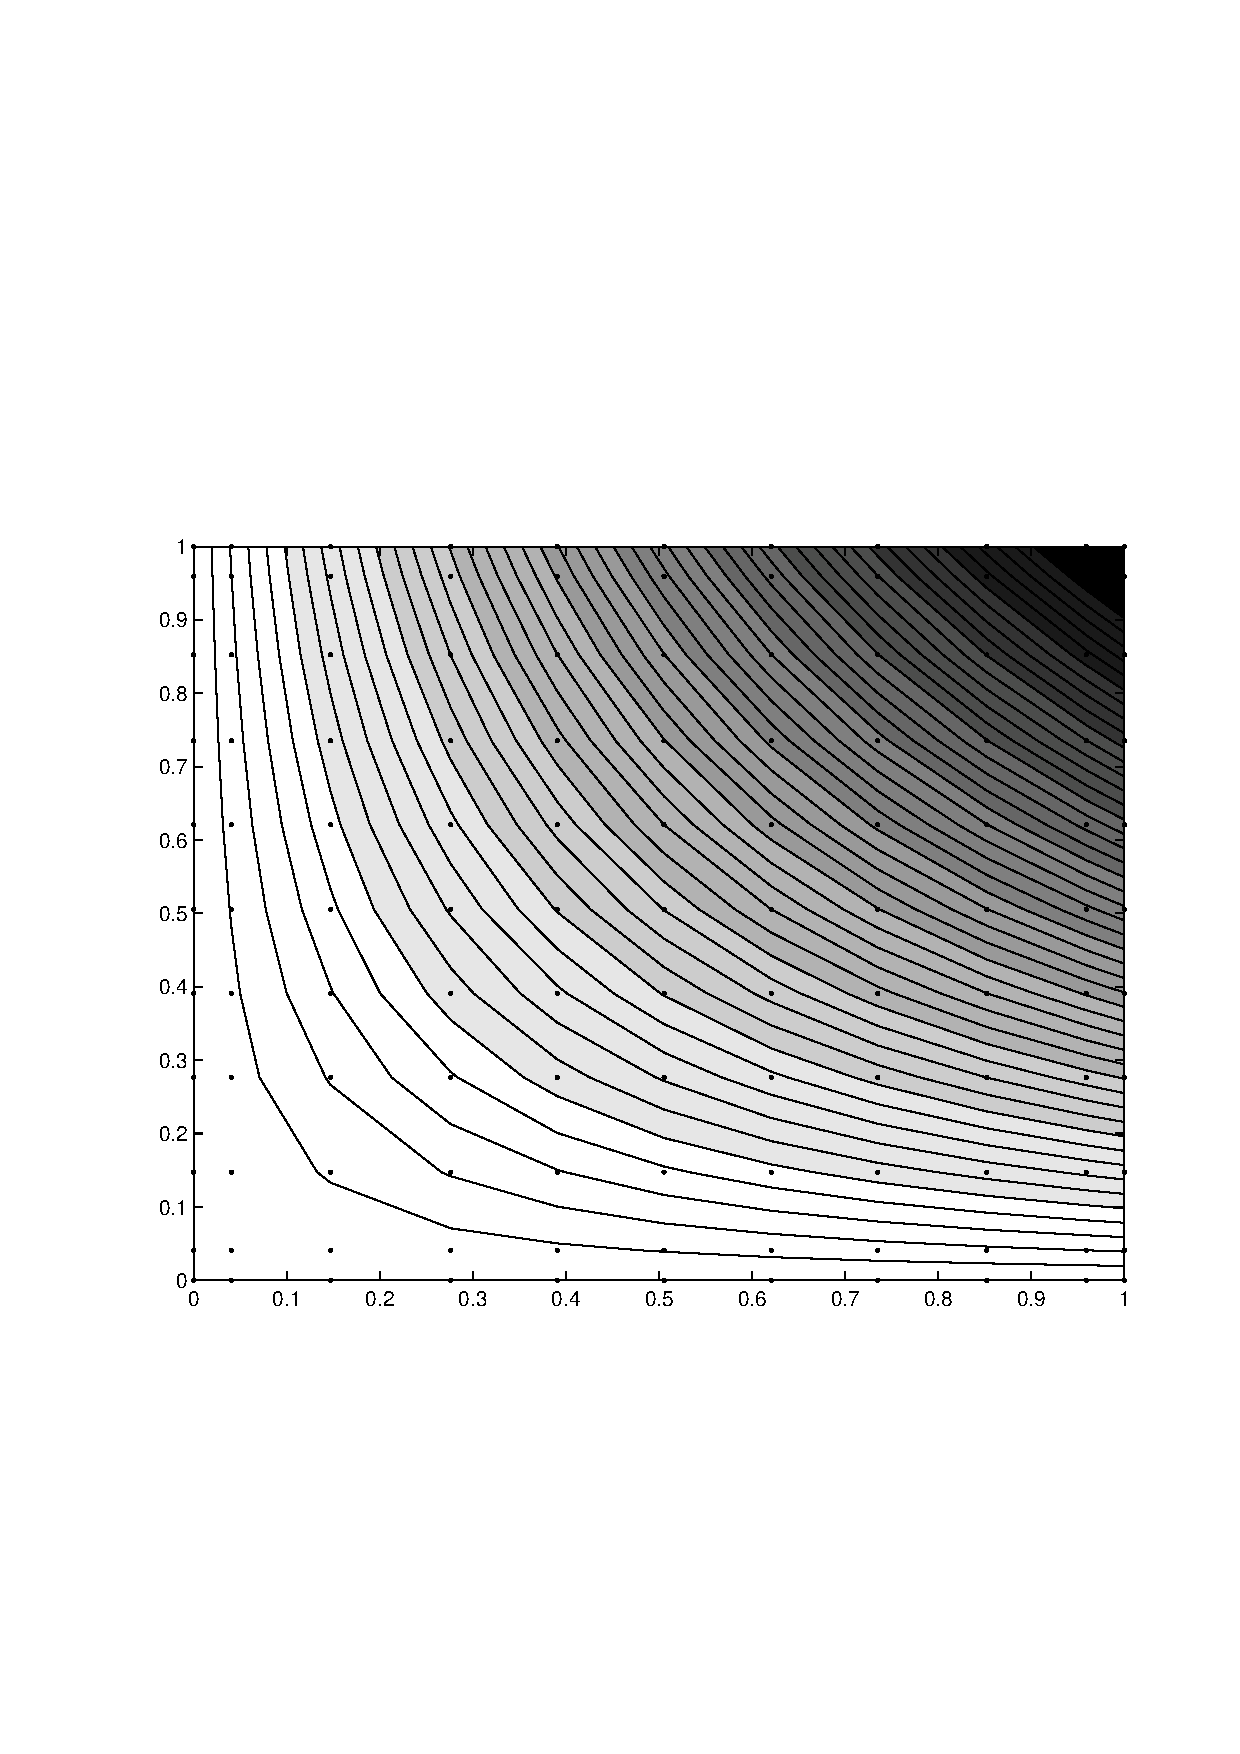
\includegraphics[scale=0.45, trim = 30mm 75mm 15mm 80mm, clip]{./Figures/3-BVP/results_10.pdf}
\caption{Isolines of the $u$ function in the square domain [0,1]x[0,1], 10x10
points.
}
\end{figure}


\columnbreak

\begin{figure}[H]
\centering
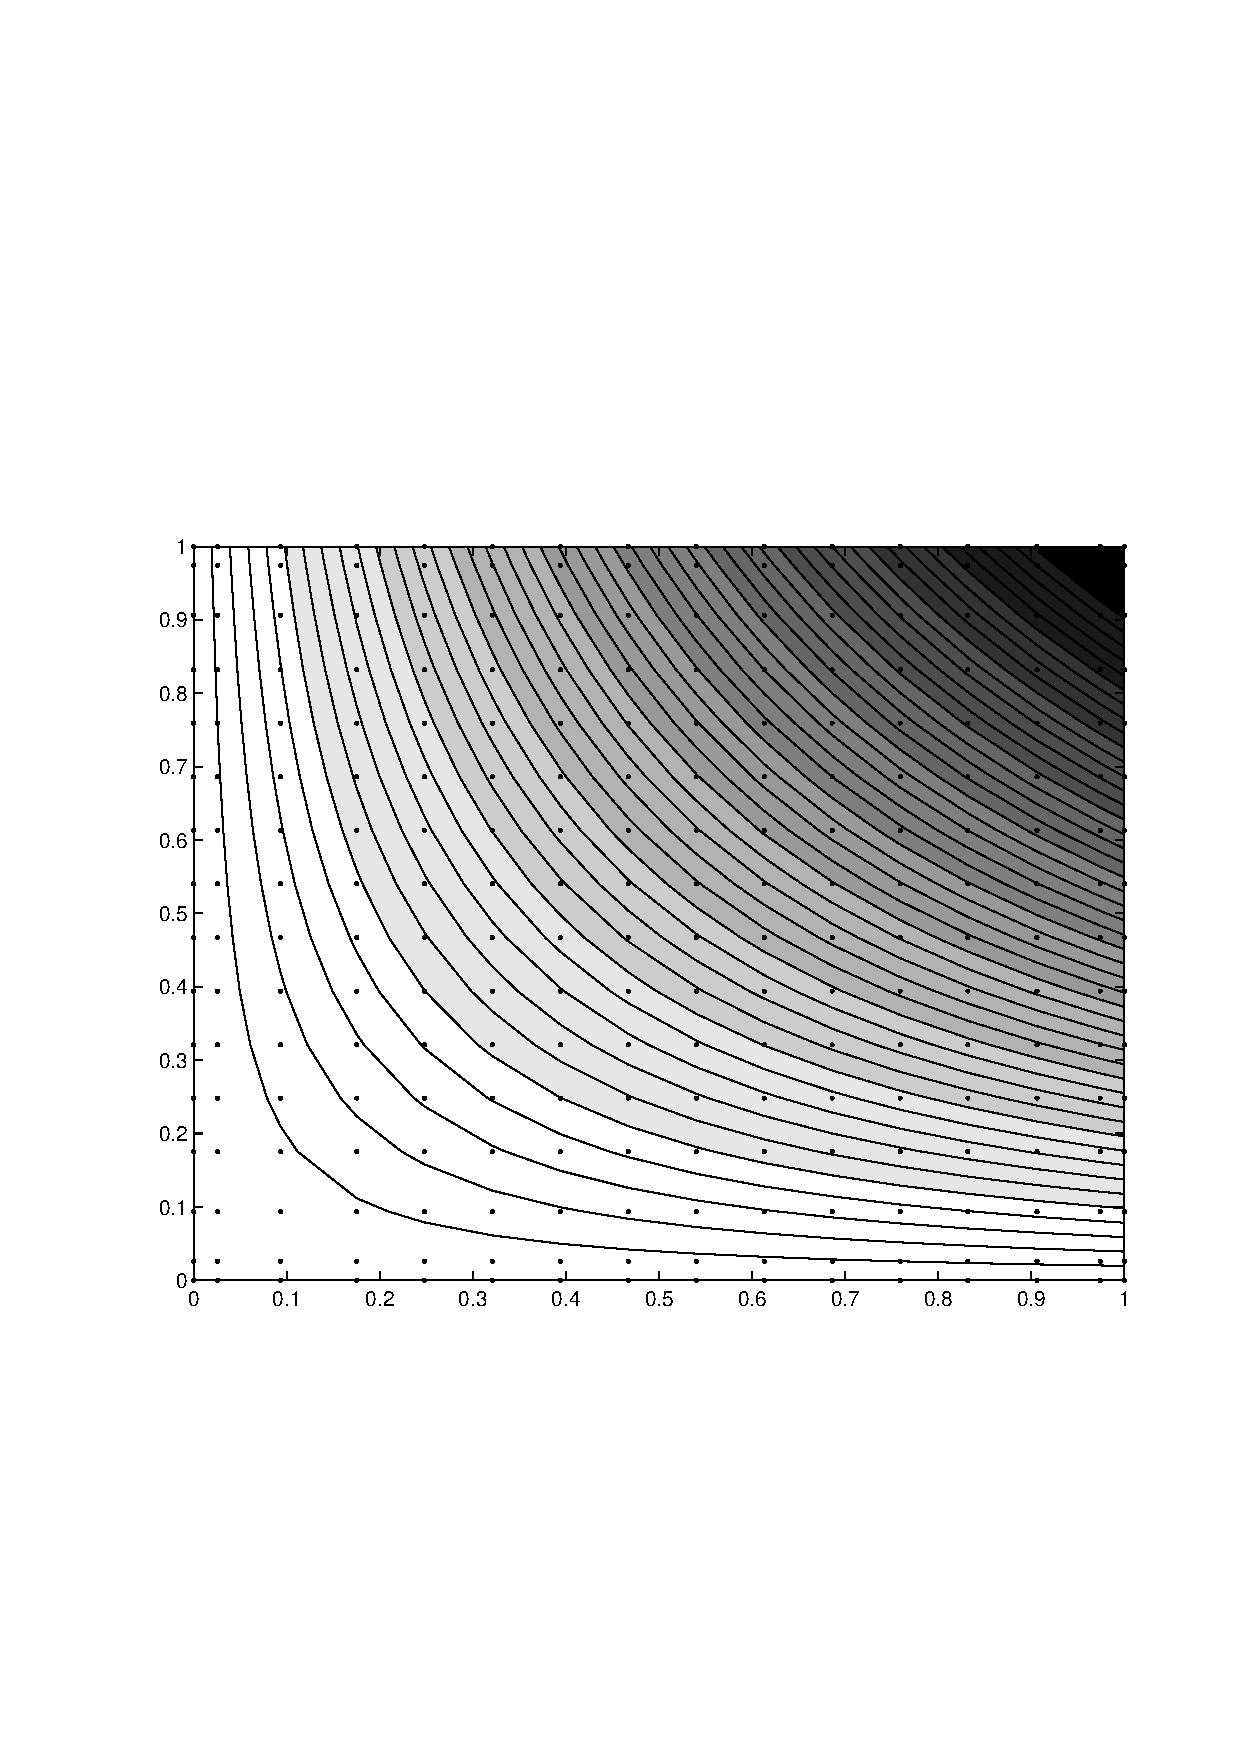
\includegraphics[scale=0.45, trim = 30mm 75mm 15mm 80mm, clip]{./Figures/3-BVP/results_15.pdf}
\caption{Isolines of the $u$ function in the square domain [0,1]x[0,1], 15x15
points. }
\end{figure}

\end{multicols}

\begin{multicols}{2}

\begin{figure}[H]
\centering
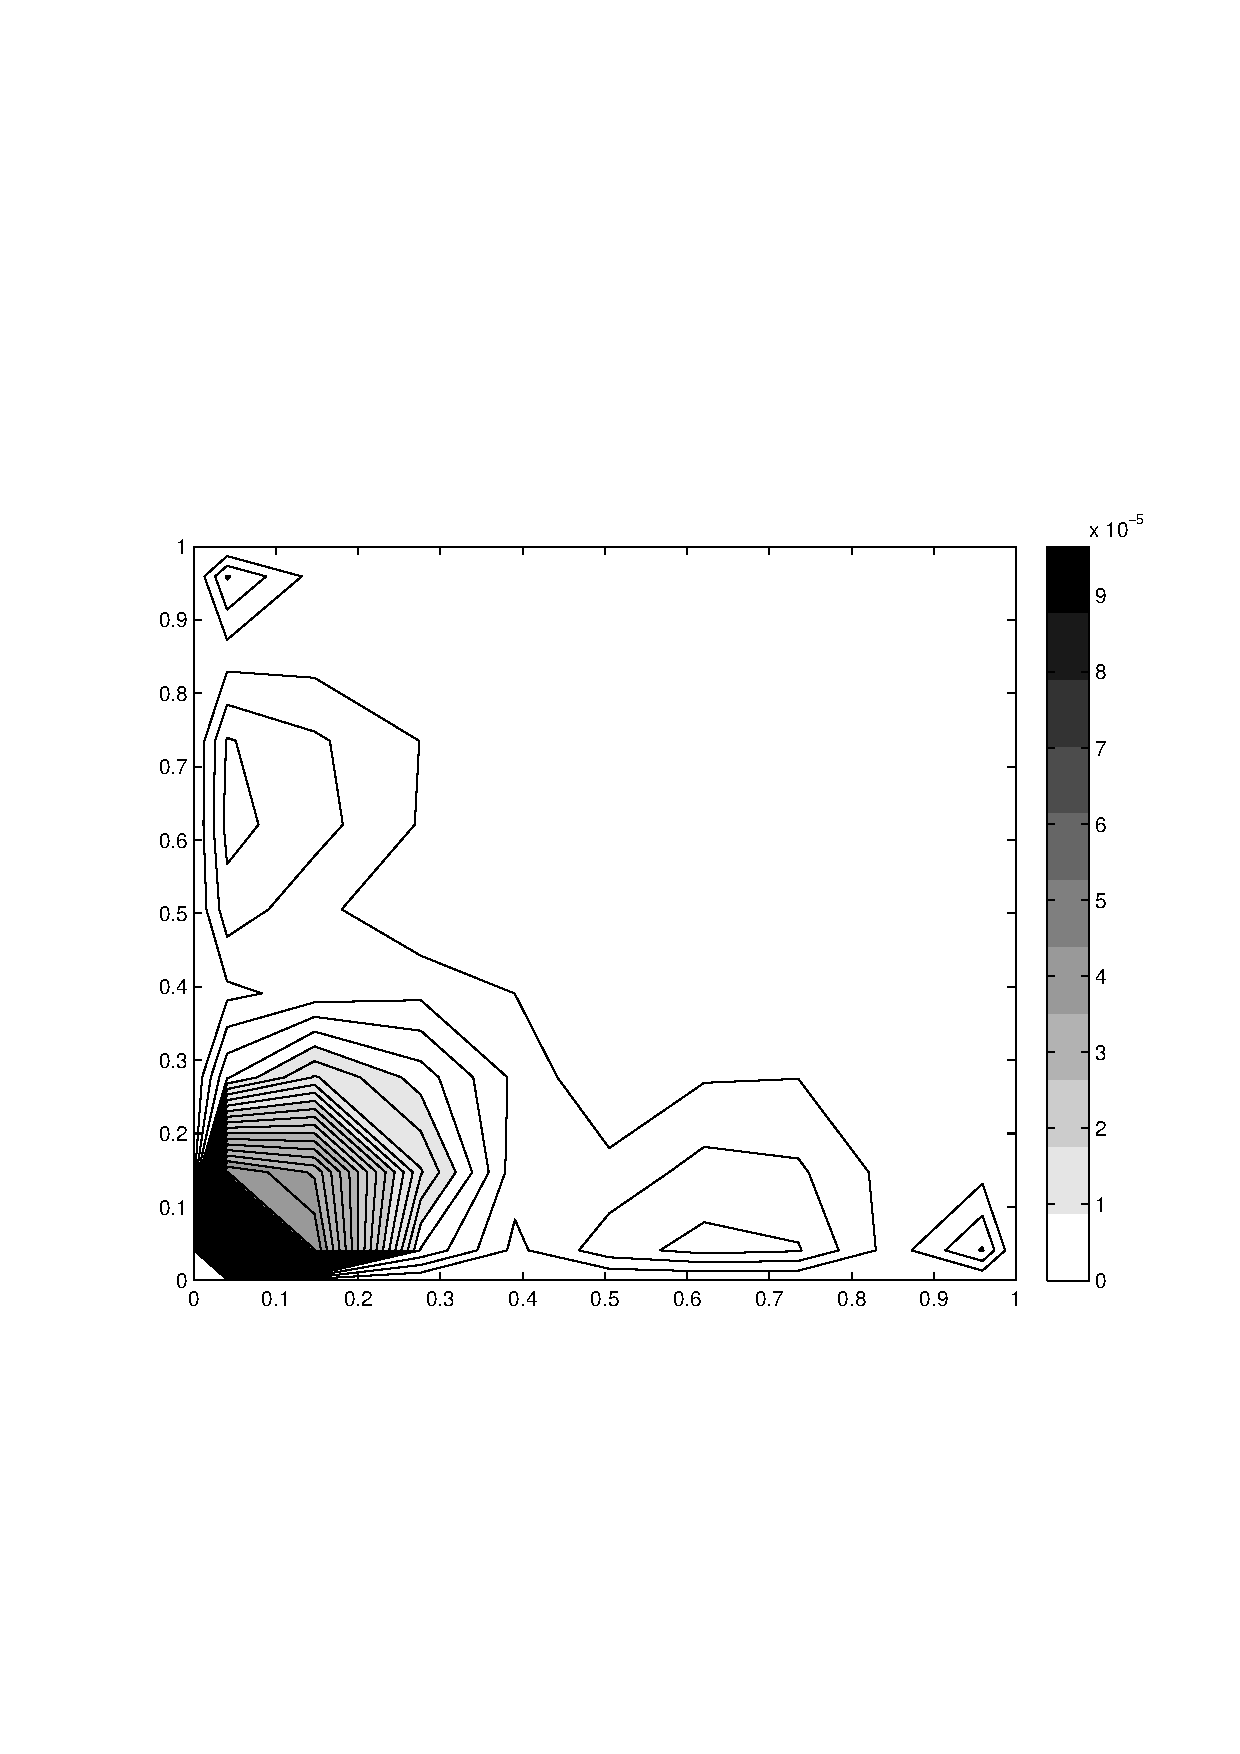
\includegraphics[scale=0.45, trim = 30mm 75mm 15mm 70mm, clip]{./Figures/3-BVP/error_10.pdf}
\caption{Comparison with the exact solution $Error=u_{ij}-x\cdot y$, 10x10
points.}
\end{figure}


\columnbreak

\begin{figure}[H]
\centering
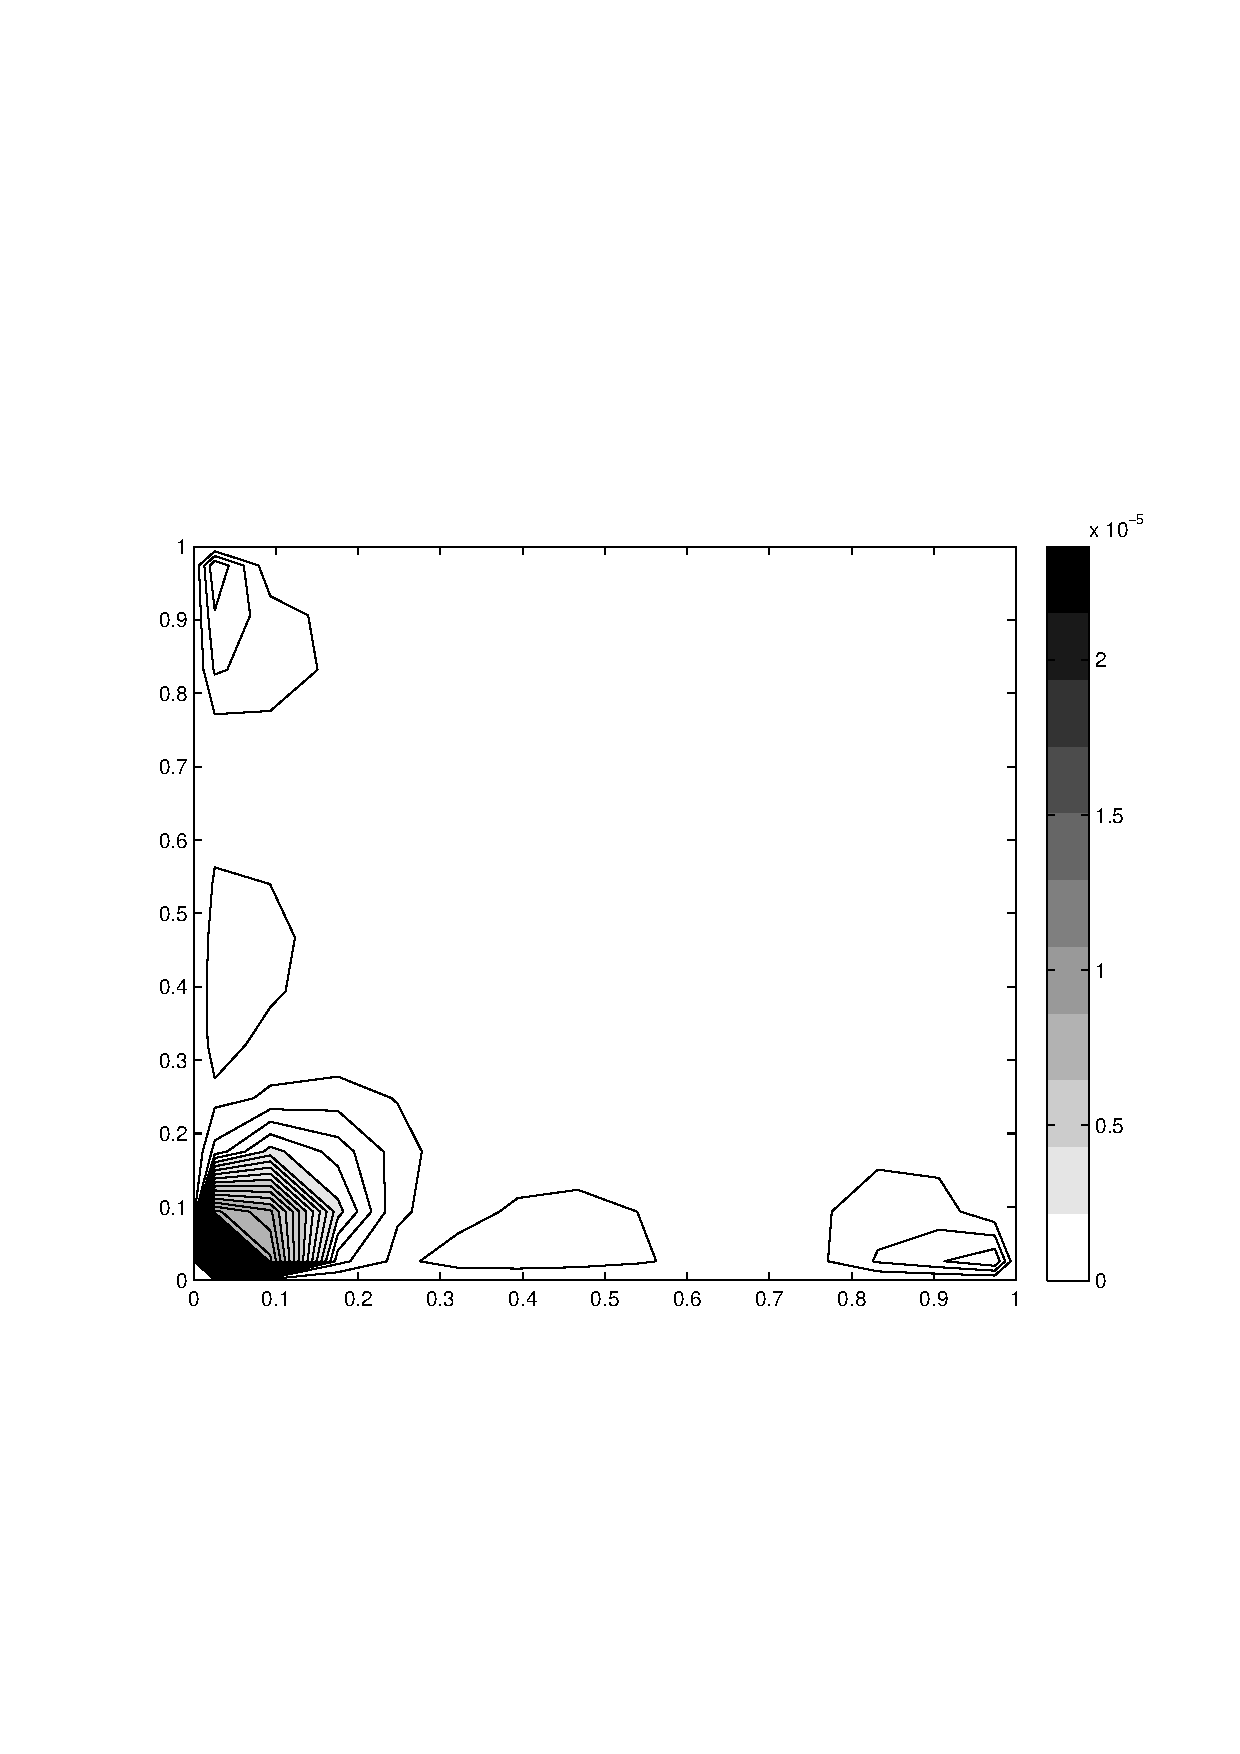
\includegraphics[scale=0.45, trim = 30mm 75mm 15mm 70mm, clip]{./Figures/3-BVP/error_15.pdf}
\caption{Comparison with the exact solution $Error=u_{ij}-x\cdot y$, 15x15
points. }
\end{figure}

\end{multicols}



The software application for this problem is presented now. A good practise
could be to check the solution of the numerical application with different
initial points for the iteration (or even using a different solver defined by
the reader).\\

\begin{blueframed}
\begin{lstlisting}
subroutine Test_non_linear_BVP_4

       use dislin

       integer, parameter :: Nx = 10, Ny = 10
       real :: x(0:Nx), y(0:Ny), U(0:Nx, 0:Ny), err(0:Nx, 0:Ny)

       integer :: i, j
       real :: a=0, b=1
       real :: pi = 4 * atan(1.0)


       x = [ (a + (b-a)*i/Nx, i=0, Nx) ]
       y = [ (a + (b-a)*j/Ny, j=0, Ny) ]

       
        do i=0, Nx
           U(i,:) = 1
     	enddo



      call Non_Linear_Boundary_Value_Problem( x_nodes = x,&
       y_nodes = y, Order =5, Differential_operator = Equation,&
       Boundary_conditions = BCs, Solution = U )

       write(*,*) " maxval, minval y =", maxval(y), minval(y)
       write(*,*) " maxval, minval x =", maxval(x), minval(x)
       write(*,*) " maxval, minval U =", maxval(U), minval(U)
       
       do i=0, Nx
        err(i,:) = x(i)*y(:)-U(i,:)  !numerical vs. analytical
     enddo


       call scrmod('revers')

       call qplcon( U, Nx+1, Ny+1, 20);
        call qplcon( err, Nx+1, Ny+1, 20);

contains

real function Equation(x, y, u, ux, uy, uxx, uyy, uxy)
           real, intent(in) :: x, y, u, ux, uy, uxx, uyy, uxy

        real :: pi = 4 * atan(1.0)

           Equation = (uxx+uyy)*u

end function

real function BCs(x, y, u, ux, uy)
           real, intent(in) :: x, y, u, ux, uy


   if (x==a) then
                      BCs = u
   elseif (x==b) then
                      BCs = u-y
   elseif (y==a) then
                      BCs = u
   elseif (y==b) then
                      BCs = u-x
   else
        write(*,*) " Error BCs x=", x
        write(*,*) " a, b=", a, b
        read(*,*)
   endif

end function

end subroutine

\end{lstlisting}
\end{blueframed}






